% Generated by tools/figures.mjs from analysis/position-adjust-6model-2026-10-09.json, analysis/aa-placebo-2026-10-10.json and analysis/rerun-compare-2026-10-11.json - do not edit by hand.
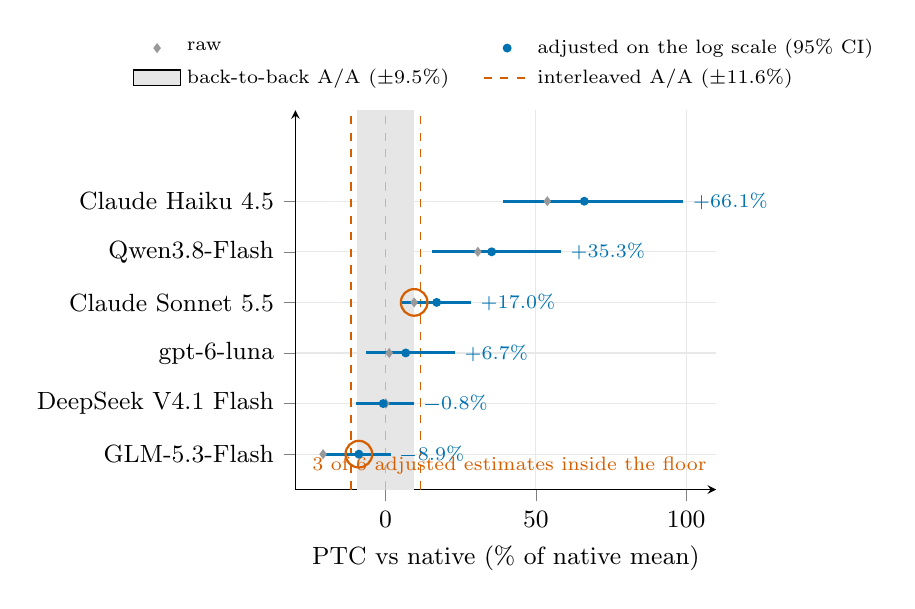
\begin{tikzpicture}
\definecolor{f4adj}{HTML}{0072B2}
\definecolor{f4raw}{HTML}{999999}
\definecolor{f4small}{HTML}{D55E00}
\begin{axis}[
  width=\linewidth-5.2cm, height=6.4cm, compat=1.18,
  xlabel={PTC vs native (\% of native mean)},
  xmin=-30, xmax=110,
  ytick={0,1,2,3,4,5},
  yticklabels={GLM-5.3-Flash,DeepSeek V4.1 Flash,gpt-6-luna,Claude Sonnet 5.5,Qwen3.8-Flash,Claude Haiku 4.5},
  ymin=-0.7, ymax=6.8,
  axis y line=left, axis x line=bottom, tick align=outside,
  grid=major, grid style={gray!18},
  yticklabel style={font=\small}, xticklabel style={font=\small}, xlabel style={font=\small}, ylabel style={font=\small},
  legend style={at={(0.5,1.03)}, anchor=south, legend columns=2, draw=none, font=\scriptsize, legend cell align=left, /tikz/every even column/.append style={column sep=10pt}},
  clip=false,
]
\addlegendimage{only marks, mark=diamond*, mark size=1.5pt, color=f4raw}
\addlegendentry{raw}
\addlegendimage{only marks, mark=*, mark size=1.4pt, color=f4adj}
\addlegendentry{adjusted on the log scale (95\% CI)}
\addlegendimage{area legend, fill=f4raw!25, draw=none}
\addlegendentry{back-to-back A/A ($\pm$9.5\%)}
\addlegendimage{f4small, dashed, line width=0.7pt}
\addlegendentry{interleaved A/A ($\pm$11.6\%)}
\fill[f4raw!25] (axis cs:-9.5,-0.7) rectangle (axis cs:9.5,6.8);
\draw[f4small, dashed, line width=0.7pt] (axis cs:-11.6,-0.7) -- (axis cs:-11.6,6.8);
\draw[f4small, dashed, line width=0.7pt] (axis cs:11.6,-0.7) -- (axis cs:11.6,6.8);
\draw[gray!55, dashed] (axis cs:0,-0.7) -- (axis cs:0,6.8);
\addplot[forget plot, only marks, mark=diamond*, mark size=1.5pt, color=f4raw] coordinates {(-20.8,0) (0.1,1) (1.2,2) (9.5,3) (30.7,4) (53.8,5)};
\addplot[forget plot, only marks, mark=*, mark size=1.4pt, color=f4adj] coordinates {(-8.9,0) (-0.8,1) (6.7,2) (17.0,3) (35.3,4) (66.1,5)};
\draw[f4adj, line width=1.1pt] (axis cs:-20.0,0) -- (axis cs:1.8,0);
\node[font=\scriptsize, anchor=west, text=f4adj] at (axis cs:1.8,0) {\textminus{}8.9\%};
\node[circle, draw=f4small, line width=0.8pt, inner sep=3.4pt] at (axis cs:-8.9,0) {};
\draw[f4adj, line width=1.1pt] (axis cs:-10.0,1) -- (axis cs:9.6,1);
\node[font=\scriptsize, anchor=west, text=f4adj] at (axis cs:9.6,1) {\textminus{}0.8\%};
\draw[f4adj, line width=1.1pt] (axis cs:-6.5,2) -- (axis cs:23.0,2);
\node[font=\scriptsize, anchor=west, text=f4adj] at (axis cs:23.0,2) {+6.7\%};
\draw[f4adj, line width=1.1pt] (axis cs:5.0,3) -- (axis cs:28.4,3);
\node[font=\scriptsize, anchor=west, text=f4adj] at (axis cs:28.4,3) {+17.0\%};
\node[circle, draw=f4small, line width=0.8pt, inner sep=3.4pt] at (axis cs:9.5,3) {};
\draw[f4adj, line width=1.1pt] (axis cs:15.6,4) -- (axis cs:58.3,4);
\node[font=\scriptsize, anchor=west, text=f4adj] at (axis cs:58.3,4) {+35.3\%};
\draw[f4adj, line width=1.1pt] (axis cs:39.1,5) -- (axis cs:99.1,5);
\node[font=\scriptsize, anchor=west, text=f4adj] at (axis cs:99.1,5) {+66.1\%};
\node[font=\scriptsize, anchor=south east, text=f4small] at (axis cs:110,-0.6) {3 of 6 adjusted estimates inside the floor};
\end{axis}
\end{tikzpicture}
